\section{World to image plane}
\label{sec:wrd2cam}
Accordingly with what we reported in Section \ref{sec:pinhole_camera}, the second step is to determine the 3D point coordinates in a reference system concordant with the image plane. The plane of interest $S$ is a plane parallel with lens plane and passing through the plane parallel to the sensor.  This choice is due to the possibility to tilt the lens with respect to the sensor, accordingly with the Scheimpflug principle, described above. If we consider the image plane parallel to the sensor directly, some issue arises. Tilting the lens changes the focal length of the camera, that varies point by point, resulting in a distorted image. This problem can be simplified observing that if we tilt the lens, we add an image plane rotated with respect to the classical image plane. In this way, the transformation between the two planes is a simple projection between planes. So we decided to split the problem in two subproblems: the first, described in this section, requires to change coordinates reference system; the second, described in Section \ref{sec:scheimflug}, needs to project the point on a different plane. Furthermore, this choice allows to simplify the mathematical model. \\

Let's focus on the Figure \ref{fig:laser-triang-a}.
  \begin{figure}[t!]
    \centering
    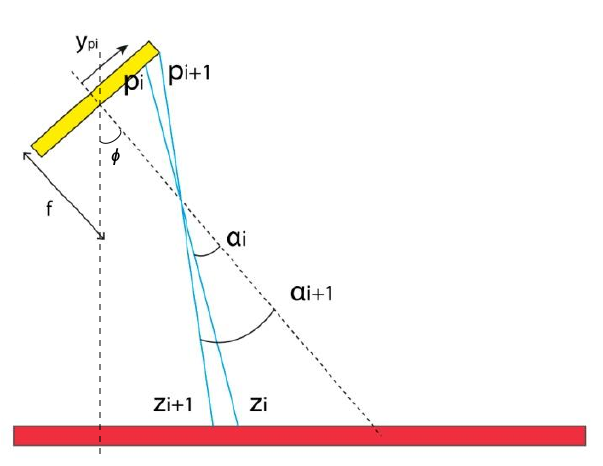
\includegraphics[width=0.7\textwidth]{./images/model/laser_triang_alpha.png}
    \caption{World to image plane}
    \label{fig:laser-triang-a}
  \end{figure}
As we can see, a change in the 3D point coordinates causes a variation in the image plane. However this alterations deals with the angle $\alpha$, estimated as offset from the triangulation angle $\phi$. Furthermore, laser plane and image plane are not parallel: this means that the two variations are different. What we are interested in, is the variation on the image plane, not in the world, so we can formulate this problem, accordingly with \cite{th:quattrini}, as:
  \begin{equation}
  	\alpha_i = \arctan\left( \frac{y_{s_i}}{f} \right)
    \label{eq:model:alpha}
  \end{equation}
where $y_{s_i}$ is the $i^{th}$ points in the image plane $S$. Being careful, it is simple to observe that the same relation is valid when determining the error due evaluating the $x$ coordinate, but with respect to the optical axis:
  \begin{equation*}
  	\beta_i = \arctan\left( \frac{x_{s_i}}{f} \right)
  \end{equation*}
Note that this step is important also to determine the natural camera resolution, in fact it allows to define the minimum variation appreciated by the sensor while it is observing the world.

So we can conclude writing that:
  \begin{equation}
    \label{eq:det_a}
  	\sigma_{\alpha_i} = \sqrt{
  	  \left( \frac{\partial \alpha_i}{\partial y_{s_i}} \right)^2 \sigma_{y_{s_i}}^2
  	  + \left( \frac{\partial \alpha_i}{\partial f} \right)^2 \sigma_f^2
  	}
  \end{equation} \\

Also in this case, $f$ is a parameter estimated thanks to the calibration processes, so we can consider it as negligible. Then, we can simplify Equation \ref{eq:det_a} as
  \begin{equation*}
  	\sigma_{\alpha_i} = \sqrt{
  	  \left( \frac{\partial \alpha_i}{\partial y_{s_i}} \right)^2 \sigma_{y_{s_i}}^2
  	}
  \end{equation*}
The same conclusions can be applied to $\beta_i$. \\

As we will see later, this transformation is the most delicate one, probably because of the change of reference system. In fact we can consider it as a passage from 3D to 2D reference system.
